\documentclass[a4paper]{exam}

\usepackage{amsmath,geometry,graphicx,hyperref,titling}
\usepackage{tikz} % Import the tikz package
\usetikzlibrary{automata} % Import library for drawing automata
\usetikzlibrary{positioning} % ...positioning nodes
\usetikzlibrary{arrows} % ...customizing arrows
\tikzset{node distance=2.5cm, % Minimum distance between two nodes. Change if necessary.
every state/.style={ % Sets the properties for each state
semithick,
fill=gray!10},
initial text={}, % No label on start arrow
double distance=2pt, % Adjust appearance of accept states
every edge/.style={ % Sets the properties for each transition
draw,
->,>=stealth', % Makes edges directed with bold arrowheads
auto,
semithick}}

\newcommand*\primary{\textsuperscript{0}}

% Header and footer.
\pagestyle{headandfoot}
\runningheadrule
\runningfootrule
\runningheader{CS 212, Fall 2022}{WC 08: Decidability}{\theauthor}
\runningfooter{}{Page \thepage\ of \numpages}{}
\firstpageheader{}{}{}

\printanswers

\title{Weekly Challenge 08: Decidability}
\author{mq06861} % <=== replace with your student ID, e.g. xy012345
\date{CS 212 Nature of Computation\\Habib University\\Fall 2022}

\qformat{{\large\bf \thequestion. \thequestiontitle}\hfill}
\boxedpoints

\begin{document}
\maketitle

\begin{questions}
	
\titledquestion{Deciding Palindromes}

	Show that determining whether a given string over $\{0,1\}$ is a palindrome is a decidable problem.

You may proceed as follows. All references below are from the textbook.
\begin{parts}
\part Formulate the problem in terms of membership in a language. For example, see the languages $D$ and $D_1$ in the subsection ``Hilbert’s Problems'' on Page 182.
\part Show that this language is Turing-decidable (see Definition 3.6) by giving a Turing machine algorithm that decides it. You may provide \textit{formal}, \textit{implementation}, or \textit{high-level} descriptions of the algorithm (see ``Terminology for describing Turing Machines'' on Page 184). For example, formal descriptions are given in Examples 3.7 and 3.9, implementation descriptions are given in Examples 3.7, 3.11 and 3.12, and a high-level description is given in Example 3.23.
\end{parts}
	
	\begin{solution}
		Let \(P=\{w\mid w\in\Sigma^*\land w=w^{\mathcal{R}}\}\). Let \(M\) be a Turing Machine which decides \(P\) in the following way. 

		\begin{enumerate}
			\item If \(w\) is empty, then \(M\) accepts.
			\item If \(w\) is not empty, then \(M\) does the following:
			\begin{enumerate}
				\item It reads the first non-empty not-\(X\) symbole replaces it with an \(X\), then it reads the last symbols and replaces it with \(X\). If they were same then \(M\) goes to step 2.
				\item If the first and last symbols of \(w\) are not the same, then \(M\) rejects.
			\end{enumerate}
		\end{enumerate}
		For low level implementation,
		\begin{center}
			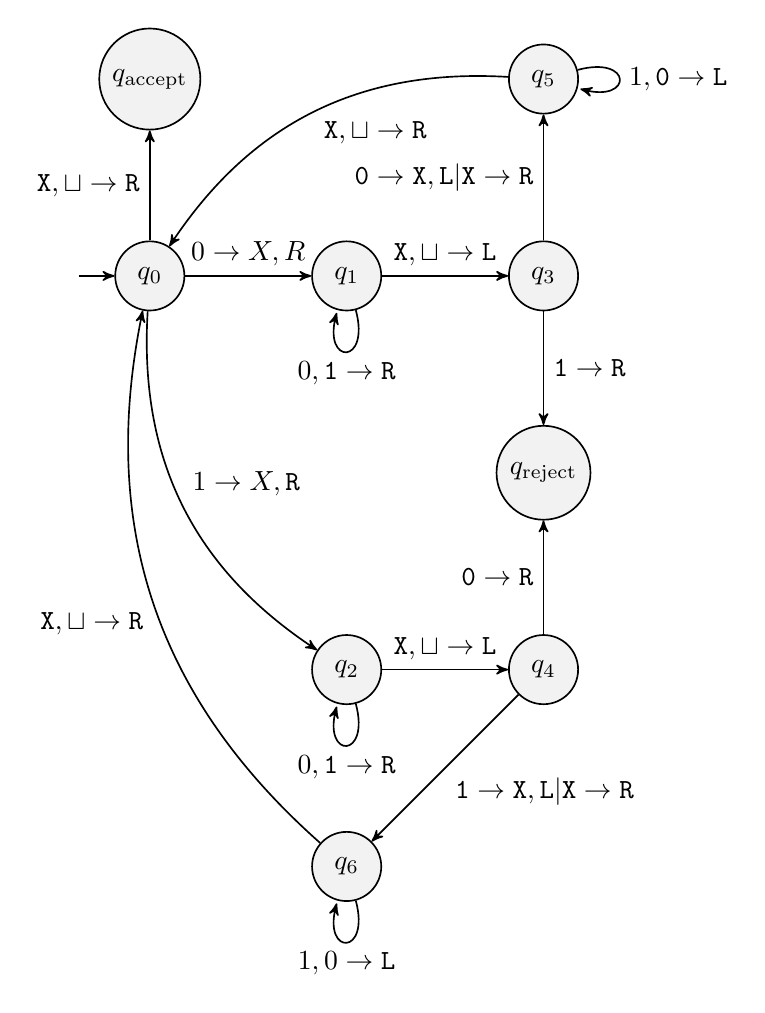
\begin{tikzpicture}
				\node[state, initial] (q0) {$q_0$};
				\node[state, right of=q0] (q1) {$q_1$};
				\node[state, right of=q1] (q3) {$q_3$};
				\node[state, above of=q3] (q5) {$q_5$};
				\node[state, above of=q0] (q7) {$q_\text{accept}$};
				\node[state, below of=q3] (q8) {$q_\text{reject}$};
				\node[state, below of=q8] (q4) {$q_4$};
				\node[state, left of=q4] (q2) {$q_2$};
				\node[state, below of=q2] (q6) {$q_6$};

				\draw (q0) edge node {$\tt X,\sqcup\to R$} (q7);
				\draw (q0) edge node {$0\to X,R$} (q1);

				\draw (q1) edge[loop below] node {$0,\tt 1\to R$} (q1);
				\draw (q1) edge node {$\tt X,\sqcup\to L$} (q3);

				\draw (q3) edge node {$\tt 0\to X,L|X\to R$} (q5);
				\draw (q5) edge[loop right] node {$1,\tt 0\to L$} (q5);
				\draw (q5) edge[bend right] node {$\tt X,\sqcup\to R$} (q0);

				\draw (q0) edge[bend right] node {$1\to X,\tt R$} (q2);
				\draw (q2) edge[loop below] node {$0,\tt 1\to R$} (q2);

				\draw (q2) edge node {$\tt X, \sqcup\to L$} (q4);
				\draw (q4) edge node {$\tt 0\to R$} (q8);
				\draw (q3) edge node {$\tt 1\to R$} (q8);

				\draw (q6) edge[bend left] node {$\tt X,\sqcup\to R$} (q0);
				\draw (q4) edge node {$\tt 1\to X,L|X\to R$} (q6);
				\draw (q6) edge[loop below] node {$1,0\to \tt L$} (q6);
			\end{tikzpicture}
		\end{center}
	\end{solution}
\end{questions}
\end{document}
